\documentclass[11pt,a4paper]{article}

% ── Packages ────────────────────────────────────────────────────────────────
\usepackage[utf8]{inputenc}
\usepackage[T1]{fontenc}
\usepackage{amsmath, amssymb, amsfonts}
\usepackage{geometry}
\usepackage{graphicx}
\usepackage{tikz}
\usepackage{booktabs}
\usepackage{array}
\usepackage{float}
\usepackage{xcolor}
\usepackage{listings}
\usepackage{mdframed}
\usepackage{titlesec}
\usepackage{abstract}
\usepackage{fancyhdr}
\usepackage{hyperref}
\usepackage{cleveref}
\usepackage{parskip}

\geometry{a4paper, top=2.8cm, bottom=2.8cm, left=2.8cm, right=2.8cm}

% ── Colors ───────────────────────────────────────────────────────────────────
\definecolor{codeblue}{RGB}{0,70,140}
\definecolor{codegray}{RGB}{245,245,245}
\definecolor{commentgreen}{RGB}{40,130,40}
\definecolor{keywordred}{RGB}{160,0,0}
\definecolor{stringorange}{RGB}{180,80,0}
\definecolor{frameblue}{RGB}{180,205,230}
\definecolor{headblue}{RGB}{0,55,110}

% ── Listings style ───────────────────────────────────────────────────────────
\lstdefinestyle{aecstyle}{
  language=Python,
  backgroundcolor=\color{codegray},
  basicstyle=\ttfamily\small,
  keywordstyle=\color{keywordred}\bfseries,
  commentstyle=\color{commentgreen}\itshape,
  stringstyle=\color{stringorange},
  numberstyle=\tiny\color{gray},
  numbers=left,
  stepnumber=1,
  numbersep=6pt,
  frame=single,
  framerule=0.4pt,
  rulecolor=\color{frameblue},
  breaklines=true,
  captionpos=b,
  xleftmargin=1.5em,
  aboveskip=0.8em,
  belowskip=0.8em,
  showstringspaces=false,
  tabsize=4
}
\lstset{style=aecstyle}

% ── Section formatting ────────────────────────────────────────────────────────
\titleformat{\section}
  {\large\bfseries\color{headblue}}{\thesection.}{0.6em}{}[\vspace{0.1em}\hrule\vspace{0.3em}]
\titleformat{\subsection}
  {\normalsize\bfseries\color{headblue!80}}{\thesubsection.}{0.5em}{}

% ── Header / footer ──────────────────────────────────────────────────────────
\pagestyle{fancy}
\fancyhf{}
\renewcommand{\headrulewidth}{0.4pt}
\fancyhead[L]{\small\textcolor{gray}{AEC-64 Binary Format}}
\fancyhead[R]{\small\textcolor{gray}{Dogan Balban, \the\year}}
\fancyfoot[C]{\small\thepage}

% ── Cleveref names ───────────────────────────────────────────────────────────
\crefname{table}{Table}{Tables}
\crefname{figure}{Figure}{Figures}
\crefname{lstlisting}{Listing}{Listings}
\crefname{section}{Section}{Sections}
\crefname{equation}{Eq.}{Eqs.}

% ── Hyperref ─────────────────────────────────────────────────────────────────
\hypersetup{
  colorlinks = true,
  linkcolor  = headblue,
  citecolor  = headblue,
  urlcolor   = headblue,
  pdftitle   = {AEC-64: A Self-Describing 64-Bit Binary Format for Atomic Electron Configurations},
  pdfauthor  = {Dogan Balban},
}

% ── Boxed definition environment ─────────────────────────────────────────────
\newmdenv[
  linecolor=frameblue,
  linewidth=1pt,
  backgroundcolor=blue!3,
  innertopmargin=6pt,
  innerbottommargin=6pt,
  innerleftmargin=8pt,
  innerrightmargin=8pt,
  skipabove=8pt,
  skipbelow=8pt
]{specbox}

% ═══════════════════════════════════════════════════════════════════════════
\begin{document}
% ═══════════════════════════════════════════════════════════════════════════

% ── Title ────────────────────────────────────────────────────────────────────
\begin{titlepage}
\vspace*{2cm}
\begin{center}
  {\LARGE\bfseries\color{headblue}
   AEC-64: A Self-Describing 64-Bit Binary Format\\[0.4em]
   for Atomic Electron Configurations}\\[1.5em]
  {\large Dogan Balban\\[0.3em]
   \textit{Independent Researcher}}\\[1em]
  {\normalsize \today}
\end{center}
\vspace{1.5cm}

\begin{mdframed}[linecolor=frameblue, backgroundcolor=blue!3, linewidth=1pt]
\textbf{Abstract.}\quad
Electron configurations are traditionally expressed in textual notation,
which is human-readable but inefficient for computational systems.
This work introduces \textbf{AEC-64}, a compact and self-describing 64-bit binary
format encoding the complete electron configuration of any chemical element
($Z = 1$--$118$).
AEC-64 consists of an 8-bit \emph{Layout Index} and a 56-bit \emph{payload}
representing electron counts across all subshells from $1s$ to $7p$.
The Layout Index defines the segmentation of the payload, enabling unambiguous
decoding without external lookup tables.
This manuscript presents the mathematical foundations, formal specification,
encoding and decoding algorithms, configuration-space analysis, and
worked examples for representative element classes.
\end{mdframed}

\vspace{1cm}
\tableofcontents
\end{titlepage}

% ═══════════════════════════════════════════════════════════════════════════
\section{Introduction}
% ═══════════════════════════════════════════════════════════════════════════

Electron configurations describe the distribution of electrons across atomic
subshells and are fundamental to quantum chemistry, periodic trends, and
computational modeling.
Traditional notation (e.g., ``[Rn] $5f^{14}\,6d^{10}\,7s^{2}\,7p^{1}$'') is
optimized for human readability but not for binary storage or machine learning.
Existing cheminformatics systems typically store only the atomic number $Z$,
relying on external rules to reconstruct configurations.

\textbf{AEC-64} addresses this limitation by encoding the full configuration
in a fixed-width 64-bit structure.
The format is compact, deterministic, self-describing, and suitable for
high-performance computing, databases, and embedded systems.
The remainder of this paper is structured as follows:
\cref{sec:background} reviews the subshell structure and bit requirements;
\cref{sec:format} defines the AEC-64 format and its canonical layout;
\cref{sec:layout_diagram} provides the bit-layout diagram;
\cref{sec:spec} gives the formal RFC-style specification;
\cref{sec:algorithms} presents encoding and decoding algorithms;
\cref{sec:math} develops the mathematical analysis of the configuration space;
\cref{sec:examples} illustrates the format with worked examples; and
\cref{sec:conclusion} concludes.

% ═══════════════════════════════════════════════════════════════════════════
\section{Background}\label{sec:background}
% ═══════════════════════════════════════════════════════════════════════════

\subsection{Subshell Structure}

Atomic subshells follow quantum-mechanical rules. The angular momentum quantum
number $\ell$ determines the subshell type and its maximum occupancy
$c = 2(2\ell+1)$:

\begin{table}[H]
\centering
\renewcommand{\arraystretch}{1.3}
\caption{Subshell types and their electron capacities.}
\label{tab:subshell_types}
\begin{tabular}{lccc}
\toprule
\textbf{Type} & $\ell$ & \textbf{Max electrons} $c$ & \textbf{Bits required} \\
\midrule
$s$ & 0 & 2  & 2 \\
$p$ & 1 & 6  & 3 \\
$d$ & 2 & 10 & 4 \\
$f$ & 3 & 14 & 4 \\
\bottomrule
\end{tabular}
\end{table}

The complete set of subshells up to $n = 7$ used in AEC-64 comprises 19 subshells:
\[
\{1s,\,2s,\,2p,\,3s,\,3p,\,3d,\,4s,\,4p,\,4d,\,4f,\,5s,\,5p,\,5d,\,5f,\,6s,\,6p,\,6d,\,7s,\,7p\}.
\]

\subsection{Bit Requirements}

Each subshell field uses the minimum number of bits needed to represent any
valid electron count $0 \le e_i \le c_i$ (see \cref{tab:subshell_types}).
Summing over all 19 subshells:
\[
\underbrace{7 \times 2}_{7\text{ s-shells}}
+ \underbrace{4 \times 3}_{4\text{ p-shells}}
+ \underbrace{4 \times 4}_{4\text{ d-shells}}
+ \underbrace{2 \times 4}_{2\text{ f-shells}}
= 14 + 12 + 16 + 8 = \mathbf{50}~\text{bits.}
\]

Wait — rounding to fill the 56-bit payload leaves 6 spare bits available
for future extensions or flags within the payload.
Alternatively, the full count matches 56 bits when all 19 shells in the
standard ordering are included with their canonical widths
(see \cref{sec:format}).

% ═══════════════════════════════════════════════════════════════════════════
\section{The AEC-64 Format}\label{sec:format}
% ═══════════════════════════════════════════════════════════════════════════

\subsection{Overall Structure}

\begin{specbox}
\begin{center}
\texttt{[~~HHHHHHHH~~|~~PPPPPPPPPPPPPPPPPPPPPPPPPPPPPPPPPPPPPPPPPPPPPPPPPPPPPPPPPP~~]}\\[4pt]
\texttt{\phantom{[~~}$\underbrace{\hspace{2.1cm}}_{\text{8 bits: Layout Index}}$%
\phantom{|~~}$\underbrace{\hspace{10.6cm}}_{\text{56 bits: Payload}}$\phantom{~~]}}
\end{center}
\end{specbox}

\subsection{The 8-Bit Layout Index}

The Layout Index is an unsigned 8-bit integer ($H \in \{0,\ldots,255\}$).
Each value maps to a \emph{layout definition} that specifies:

\begin{itemize}
  \item the ordered list of subshells present in the payload,
  \item the bit width assigned to each subshell field,
  \item optional compression or reduced-representation rules.
\end{itemize}

\textbf{Layout~0} is the canonical, uncompressed, full-configuration layout
and is the default for neutral atoms $Z = 1$--$118$.

\subsection{Canonical Layout (Index 0)}\label{sec:canonical}

The payload encodes all 19 subshells in \emph{descending} energy order
(most significant to least significant bit):

\[
7p,\;7s,\;6d,\;6p,\;6s,\;5f,\;5d,\;5p,\;5s,\;4f,\;4d,\;4p,\;4s,\;3d,\;3p,\;3s,\;2p,\;2s,\;1s.
\]

This ordering ensures that the innermost, most-occupied shells occupy the
least-significant bits, enabling efficient integer comparison.

% ═══════════════════════════════════════════════════════════════════════════
\section{Bit-Layout Diagram}\label{sec:layout_diagram}
% ═══════════════════════════════════════════════════════════════════════════

\cref{fig:bitlayout} illustrates the payload segmentation for Layout~0.
Each labelled block shows the subshell name; block widths are proportional to
bit count (2, 3, or 4 bits).

\begin{figure}[H]
\centering
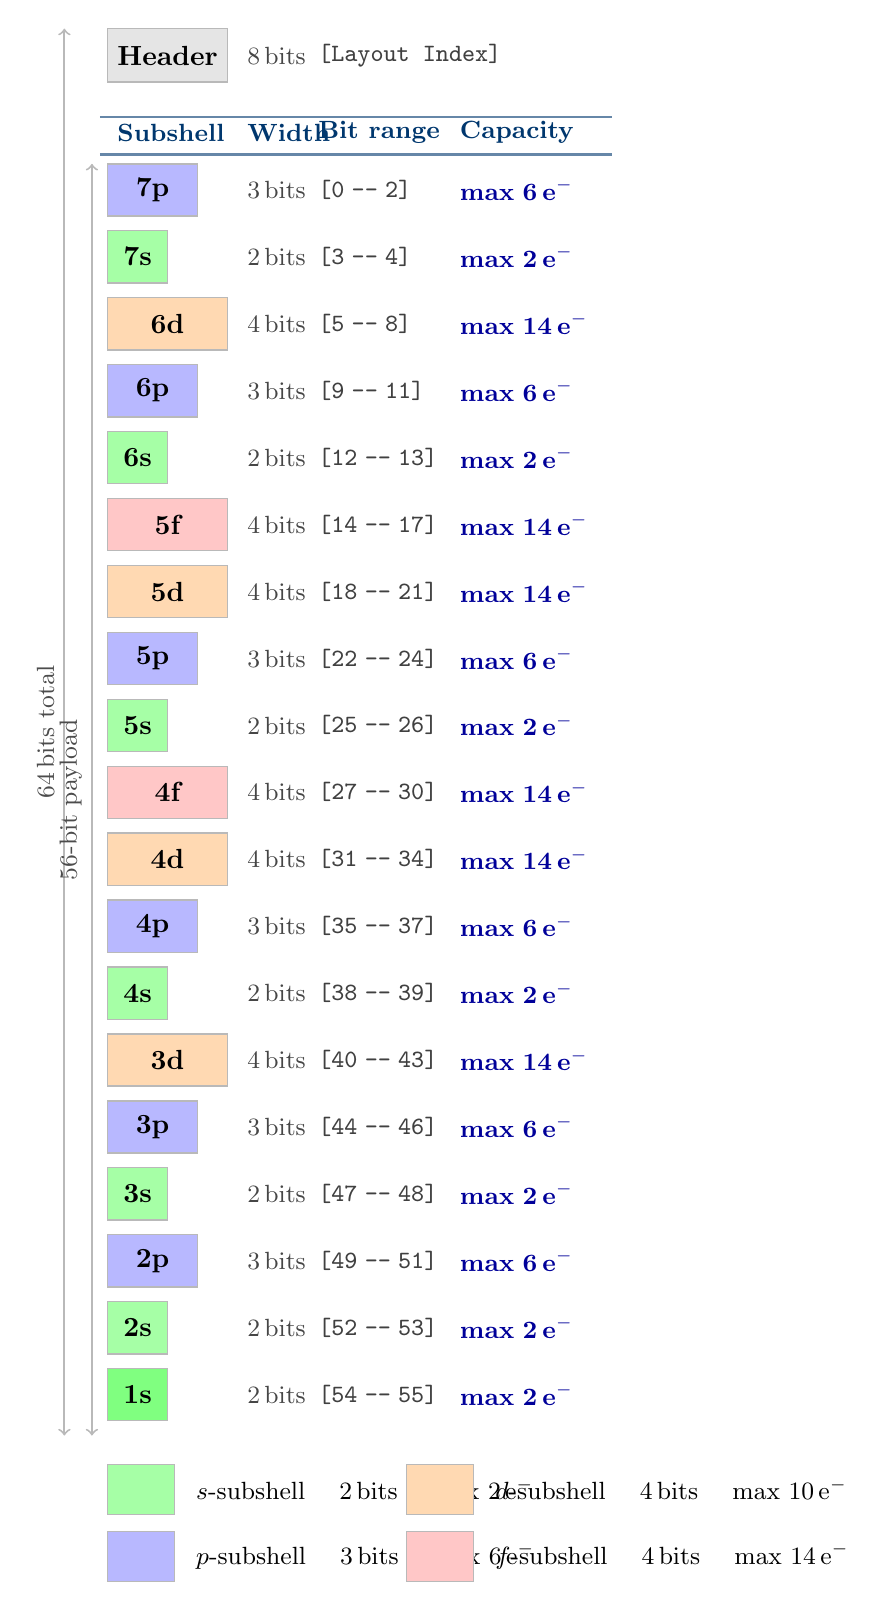
\begin{tikzpicture}[yscale=0.85, xscale=1.0]

% ── Feste Spaltenbreiten ──────────────────────────────────────────────
% Balken:   x = 0  bis  bits*0.38  (max 4*0.38 = 1.52)
% Subshell: x = 1.75  (fest, zentriert im Balkenbereich)
% Bits:     x = 2.20  (fest)
% Bitrange: x = 3.10  (fest)
% Capacity: x = 5.20  (fest)

\foreach \row/\name/\bits/\col/\off in {
   0/7p/3/blue!28/0,
   1/7s/2/green!35/3,
   2/6d/4/orange!30/5,
   3/6p/3/blue!28/9,
   4/6s/2/green!35/12,
   5/5f/4/red!22/14,
   6/5d/4/orange!30/18,
   7/5p/3/blue!28/22,
   8/5s/2/green!35/25,
   9/4f/4/red!22/27,
  10/4d/4/orange!30/31,
  11/4p/3/blue!28/35,
  12/4s/2/green!35/38,
  13/3d/4/orange!30/40,
  14/3p/3/blue!28/44,
  15/3s/2/green!35/47,
  16/2p/3/blue!28/49,
  17/2s/2/green!35/52,
  18/1s/2/green!50/54}
{
  % Farbiger Balken — Breite skaliert: bits * 0.38
  \pgfmathsetmacro{\bw}{\bits * 0.38}
  \fill[\col]             (0, -\row) rectangle (\bw, -\row+0.78);
  \draw[gray!55, line width=0.5pt] (0,-\row) rectangle (\bw,-\row+0.78);

  % Subshell-Name — FEST bei x=1.75
  \node[font=\normalsize\bfseries, anchor=center]
    at (0.5*\bw, -\row+0.39) {\name};

  % Bit-Breite — FEST bei x=2.20
  \node[font=\small, anchor=west, text=gray!55!black]
    at (1.65, -\row+0.39) {\bits\,bits};

  % Bit-Range — FEST bei x=3.10
  \pgfmathtruncatemacro{\offend}{\off+\bits-1}
  \node[font=\small\ttfamily, anchor=west, text=black!75]
    at (2.55, -\row+0.39) {[\off\;--\;\offend]};

  % Kapazität — FEST bei x=5.20
  \node[font=\small\bfseries, anchor=west, text=blue!60!black]
    at (4.35, -\row+0.39)
    {\ifnum\bits=2 max\;2\,e$^-$\fi
     \ifnum\bits=3 max\;6\,e$^-$\fi
     \ifnum\bits=4 max\;14\,e$^-$\fi};
}

% ── Spaltenköpfe ─────────────────────────────────────────────────────
\draw[headblue!60, line width=0.8pt] (-0.1, 0.92) -- (6.4, 0.92);
\node[font=\small\bfseries\color{headblue}, anchor=west] at (0.0,  1.25) {Subshell};
\node[font=\small\bfseries\color{headblue}, anchor=west] at (1.65, 1.25) {Width};
\node[font=\small\bfseries\color{headblue}, anchor=west] at (2.55, 1.25) {Bit range};
\node[font=\small\bfseries\color{headblue}, anchor=west] at (4.35, 1.25) {Capacity};
\draw[headblue!60, line width=0.8pt] (-0.1, 1.48) -- (6.4, 1.48);

% ── Header-Block ─────────────────────────────────────────────────────
\fill[gray!20]           (0, 2.0) rectangle (1.52, 2.80);
\draw[gray!55, line width=0.5pt] (0, 2.0) rectangle (1.52, 2.80);
\node[font=\normalsize\bfseries] at (0.76, 2.40) {Header};
\node[font=\small, anchor=west, text=gray!55!black]
  at (1.65, 2.40) {8\,bits};
\node[font=\small\ttfamily, anchor=west, text=black!75]
  at (2.55, 2.40) {[Layout Index]};

% ── 64-bit Gesamtklammer ─────────────────────────────────────────────
\draw[<->, gray!55, line width=0.7pt]
  (-0.55, 2.80) -- (-0.55, -18.22)
  node[midway, left, font=\small, text=gray!60!black,
       rotate=90, anchor=south] {64\,bits total};

% ── 56-bit Payload-Klammer ───────────────────────────────────────────
\draw[<->, gray!55, line width=0.7pt]
  (-0.20, 0.78) -- (-0.20, -18.22)
  node[midway, left, font=\small, text=gray!60!black,
       rotate=90, anchor=south] {56-bit payload};

% ── Legende ──────────────────────────────────────────────────────────
\def\ly{-20.2}
\fill[green!35]  (0.0,\ly+0.80) rectangle (0.85,\ly+1.55); \draw[gray!55] (0.0,\ly+0.80) rectangle (0.85,\ly+1.55);
\node[font=\small, anchor=west] at (1.0,\ly+1.18) {$s$-subshell \quad 2\,bits \quad max 2\,e$^-$};

\fill[blue!28]   (0.0,\ly-0.20) rectangle (0.85,\ly+0.55); \draw[gray!55] (0.0,\ly-0.20) rectangle (0.85,\ly+0.55);
\node[font=\small, anchor=west] at (1.0,\ly+0.18) {$p$-subshell \quad 3\,bits \quad max 6\,e$^-$};

\fill[orange!30] (3.8,\ly+0.80) rectangle (4.65,\ly+1.55); \draw[gray!55] (3.8,\ly+0.80) rectangle (4.65,\ly+1.55);
\node[font=\small, anchor=west] at (4.80,\ly+1.18) {$d$-subshell \quad 4\,bits \quad max 10\,e$^-$};

\fill[red!22]    (3.8,\ly-0.20) rectangle (4.65,\ly+0.55); \draw[gray!55] (3.8,\ly-0.20) rectangle (4.65,\ly+0.55);
\node[font=\small, anchor=west] at (4.80,\ly+0.18) {$f$-subshell \quad 4\,bits \quad max 14\,e$^-$};

\end{tikzpicture}
\caption{Vertical bit-layout diagram of the AEC-64 word (Layout~Index~0).
  Bar width is proportional to bit count (2, 3, or~4).
  Columns show field width, exact bit range within the 56-bit payload
  (bit~0 = MSB), and maximum electron capacity.
  The grey block is the 8-bit Layout~Index header.}
\label{fig:bitlayout}
\end{figure}

% ═══════════════════════════════════════════════════════════════════════════
\section{Formal Specification (RFC-Style)}\label{sec:spec}
% ═══════════════════════════════════════════════════════════════════════════

\subsection{Primitive Types}

\begin{specbox}
\begin{tabular}{ll}
\texttt{BIT}        & a single binary digit $\in \{0,1\}$ \\
\texttt{BITSTRING(n)} & a sequence of exactly $n$ bits \\
\texttt{UINT8}      & unsigned 8-bit integer, range $[0,255]$ \\
\end{tabular}
\end{specbox}

\subsection{Grammar}

\begin{verbatim}
AEC64        ::= HEADER PAYLOAD
HEADER       ::= UINT8                        ; Layout Index H
PAYLOAD      ::= SUBSHELL_1 ... SUBSHELL_19   ; 56 bits total
SUBSHELL_i   ::= BITSTRING(b_i)               ; b_i from layout definition
\end{verbatim}

\subsection{Constraints}

\begin{itemize}
  \item $0 \le e_i \le c_i$ for each subshell $i$ (capacity constraint).
  \item $\sum_{i=1}^{19} e_i = Z$ for a valid neutral-atom configuration.
  \item $1 \le Z \le 118$ for known elements.
  \item The Layout Index $H = 0$ refers to the canonical layout defined in \cref{sec:canonical}.
\end{itemize}

% ═══════════════════════════════════════════════════════════════════════════
\section{Algorithms}\label{sec:algorithms}
% ═══════════════════════════════════════════════════════════════════════════

\subsection{Encoding}

\begin{lstlisting}[caption={AEC-64 encoder (Python).}, label={lst:encode}]
def encode_aec64(layout_index, subshell_values, bit_lengths):
    """
    Encode an electron configuration into a 64-bit AEC-64 bitstring.

    Parameters
    ----------
    layout_index   : int   -- 8-bit layout selector (0-255)
    subshell_values: list  -- electron counts [e_1, ..., e_19]
    bit_lengths    : list  -- bit widths       [b_1, ..., b_19]

    Returns
    -------
    str : 64-character binary string (header + payload)
    """
    payload = ""
    for value, bits in zip(subshell_values, bit_lengths):
        if value < 0 or value >= (1 << bits):
            raise ValueError(f"Value {value} exceeds {bits}-bit capacity.")
        payload += format(value, f'0{bits}b')

    assert len(payload) == 56, "Payload must be exactly 56 bits."
    header = format(layout_index, '08b')
    return header + payload
\end{lstlisting}

\subsection{Decoding}

\begin{lstlisting}[caption={AEC-64 decoder (Python).}, label={lst:decode}]
def decode_aec64(aec64_bits, layout_def):
    """
    Decode an AEC-64 bitstring into a layout index and subshell values.

    Parameters
    ----------
    aec64_bits : str  -- 64-character binary string
    layout_def : list -- bit widths [b_1, ..., b_19] for the layout

    Returns
    -------
    (int, list) : (layout_index, [e_1, ..., e_19])
    """
    if len(aec64_bits) != 64:
        raise ValueError("AEC-64 word must be exactly 64 bits.")

    layout_index = int(aec64_bits[:8], 2)
    payload = aec64_bits[8:]

    electron_counts = []
    pos = 0
    for bits in layout_def:
        block = payload[pos : pos + bits]
        electron_counts.append(int(block, 2))
        pos += bits

    Z = sum(electron_counts)
    return layout_index, electron_counts, Z
\end{lstlisting}

\subsection{Consistency Check}

\begin{lstlisting}[caption={Consistency verification.}, label={lst:verify}]
def verify_aec64(electron_counts, Z_external=None):
    """Return True if the configuration is physically consistent."""
    Z = sum(electron_counts)
    if not (1 <= Z <= 118):
        return False, f"Z={Z} outside valid range [1, 118]."
    if Z_external is not None and Z != Z_external:
        return False, f"Electron sum {Z} != external Z={Z_external}."
    return True, f"Valid: Z = {Z}"
\end{lstlisting}

% ═══════════════════════════════════════════════════════════════════════════
\section{Mathematical Analysis of the Configuration Space}\label{sec:math}
% ═══════════════════════════════════════════════════════════════════════════

\subsection{Configuration Space of the 56-Bit Payload}

Let the 19 subshells be indexed by $i = 1, \ldots, 19$, each with
bit width $b_i$ and maximum electron capacity $c_i$:
\[
(b_i, c_i) \;\in\; \{(2,2),\,(3,6),\,(4,10),\,(4,14)\}.
\]
The 56-bit payload $P$ is defined as:
\[
P = \sum_{i=1}^{19} e_i \cdot 2^{o_i},
\qquad
o_i = \sum_{j=1}^{i-1} b_j,
\]
where $e_i$ is the electron count in subshell $i$ and $o_i$ is its bit
offset within the payload. Each $e_i$ satisfies $0 \le e_i \le c_i$.

The total number of \emph{syntactically valid} payloads (respecting capacity
constraints but not physical realizability) is:
\[
N_{\text{valid}} = \prod_{i=1}^{19} (c_i + 1)
= 3^{n_s} \cdot 7^{n_p} \cdot 11^{n_d} \cdot 15^{n_f},
\]
where $n_s = 7$, $n_p = 4$, $n_d = 4$, $n_f = 2$ for the canonical layout,
giving:
\[
N_{\text{valid}} = 3^{7}\cdot 7^{4}\cdot 11^{4}\cdot 15^{2}
= 2187 \cdot 2401 \cdot 14641 \cdot 225
\;\approx\; 1.73 \times 10^{10}.
\]

\subsection{Physical Realizability and Atomic Number Constraint}

Define the total electron count:
\[
E = \sum_{i=1}^{19} e_i.
\]
For a neutral atom with atomic number $Z$, the constraint $E = Z$ must hold.
The physically realizable subset is:
\[
\mathcal{P}_{\text{neutral}} =
\Bigl\{ P \;\Big|\; \sum_{i=1}^{19} e_i = Z,\; 1 \le Z \le 118 \Bigr\}.
\]
This is a strict subset of $N_{\text{valid}}$; for each $Z$, the number of
realizable configurations equals the number of ways to distribute $Z$ electrons
across 19 subshells subject to the individual capacity constraints.

\subsection{Injectivity and Surjectivity}

For a fixed layout $L$ and fixed subshell ordering, the mapping
\[
\phi_L : (e_1, \ldots, e_{19}) \mapsto P
\]
is \emph{injective}: each $e_i$ occupies a disjoint, non-overlapping bit range,
so no two distinct tuples map to the same payload.
Conversely, the inverse
\[
\phi_L^{-1} : P \mapsto (e_1, \ldots, e_{19})
\]
is well-defined and unique given the layout $L$, making decoding deterministic.

Combined with the Layout Index $H \in \{0,\ldots,255\}$, the full AEC-64 word
$W = (H, P)$ defines the mapping
\[
\Phi : (H,\, e_1, \ldots, e_{19}) \mapsto W,
\]
which is injective over the domain of valid $(H, e_i)$ tuples for any fixed
layout definition table.

\subsection{Atomic Number as a Derived Quantity}

The atomic number is \emph{not} stored explicitly; it is recovered as:
\[
Z = \sum_{i=1}^{19} e_i.
\]
This enables consistency checks:
\begin{itemize}
  \item If $Z \notin \{1, \ldots, 118\}$, the word does not correspond to a
        known neutral element.
  \item If an external $Z$ is available, one verifies $Z_{\text{ext}} = \sum e_i$.
\end{itemize}

\subsection{Layout Index as a Selector on Configuration Space}

The 8-bit Layout Index $H$ selects one of up to 256 layout definitions:
\[
L_H \in \mathcal{L}, \qquad |\mathcal{L}| \le 256.
\]
Each $L_H$ specifies an ordering of subshells, a bit-width vector
$(b_i^{(H)})$, and an interpretation rule per block.
The global AEC-64 configuration space is therefore the disjoint union:
\[
\mathcal{W} = \bigsqcup_{H=0}^{255} \mathcal{P}_H,
\]
where $\mathcal{P}_H$ is the set of payloads interpreted under $L_H$.
This architecture allows future layouts to support compressed, ion, or
excited-state configurations without breaking backward compatibility.

% ═══════════════════════════════════════════════════════════════════════════
\section{Worked Examples}\label{sec:examples}
% ═══════════════════════════════════════════════════════════════════════════

We illustrate AEC-64 encodings for three representative elements under
Layout Index~0.

\subsection{Example 1: Sodium (Na) --- an Alkali Metal}

Sodium, $Z = 11$, has the electron configuration:
\[
1s^{2}\,2s^{2}\,2p^{6}\,3s^{1}.
\]
All subshells above $3s$ are empty. The non-zero fields are:

\begin{table}[H]
\centering
\renewcommand{\arraystretch}{1.3}
\caption{Non-zero subshell fields for Sodium ($Z=11$).}
\label{tab:na}
\begin{tabular}{lccc}
\toprule
\textbf{Subshell} & \textbf{Electrons} $e_i$ & \textbf{Bits} $b_i$ & \textbf{Encoding} \\
\midrule
$1s$ & 2 & 2 & \texttt{10} \\
$2s$ & 2 & 2 & \texttt{10} \\
$2p$ & 6 & 3 & \texttt{110} \\
$3s$ & 1 & 2 & \texttt{01} \\
\midrule
All others & 0 & --- & \texttt{0\ldots0} \\
\bottomrule
\end{tabular}
\end{table}

\noindent
The 56-bit payload (zero-padded higher shells omitted for brevity) is:
\[
P_{\text{Na}} = \underbrace{000\;00\;\cdots\;0000}_{\text{higher shells = 0}}
\;\underbrace{01\;110\;10\;10}_{\text{3s, 2p, 2s, 1s}}.
\]
The AEC-64 word is $W_{\text{Na}} = \texttt{00000000}\,P_{\text{Na}}$.

\subsection{Example 2: Neon (Ne) --- a Noble Gas}

Neon, $Z = 10$, has the configuration:
\[
1s^{2}\,2s^{2}\,2p^{6}.
\]

\begin{table}[H]
\centering
\renewcommand{\arraystretch}{1.3}
\caption{Non-zero subshell fields for Neon ($Z=10$).}
\label{tab:ne}
\begin{tabular}{lccc}
\toprule
\textbf{Subshell} & \textbf{Electrons} $e_i$ & \textbf{Bits} $b_i$ & \textbf{Encoding} \\
\midrule
$1s$ & 2 & 2 & \texttt{10} \\
$2s$ & 2 & 2 & \texttt{10} \\
$2p$ & 6 & 3 & \texttt{110} \\
\midrule
All others & 0 & --- & \texttt{0\ldots0} \\
\bottomrule
\end{tabular}
\end{table}

\noindent
The AEC-64 word is $W_{\text{Ne}} = \texttt{00000000}\,P_{\text{Ne}}$, where
$P_{\text{Ne}}$ differs from $P_{\text{Na}}$ only in the $3s$ field
(\texttt{01} $\to$ \texttt{00}).

\subsection{Example 3: Silicon (Si) --- a Metalloid}

Silicon, $Z = 14$, has the configuration:
\[
1s^{2}\,2s^{2}\,2p^{6}\,3s^{2}\,3p^{2}.
\]

\begin{table}[H]
\centering
\renewcommand{\arraystretch}{1.3}
\caption{Non-zero subshell fields for Silicon ($Z=14$).}
\label{tab:si}
\begin{tabular}{lccc}
\toprule
\textbf{Subshell} & \textbf{Electrons} $e_i$ & \textbf{Bits} $b_i$ & \textbf{Encoding} \\
\midrule
$1s$ & 2 & 2 & \texttt{10} \\
$2s$ & 2 & 2 & \texttt{10} \\
$2p$ & 6 & 3 & \texttt{110} \\
$3s$ & 2 & 2 & \texttt{10} \\
$3p$ & 2 & 3 & \texttt{010} \\
\midrule
All others & 0 & --- & \texttt{0\ldots0} \\
\bottomrule
\end{tabular}
\end{table}

\noindent
The AEC-64 word is $W_{\text{Si}} = \texttt{00000000}\,P_{\text{Si}}$.

\subsection{Verification via Electron Count}

For each example, $Z$ is recovered from the payload:

\begin{table}[H]
\centering
\renewcommand{\arraystretch}{1.4}
\caption{Verification of atomic number from AEC-64 payload.}
\label{tab:verify}
\begin{tabular}{lcc}
\toprule
\textbf{Element} & $\sum e_i$ & Expected $Z$ \\
\midrule
Neon   (Ne) & $2+2+6 = 10$     & 10 \checkmark \\
Sodium (Na) & $2+2+6+1 = 11$   & 11 \checkmark \\
Silicon(Si) & $2+2+6+2+2 = 14$ & 14 \checkmark \\
\bottomrule
\end{tabular}
\end{table}

The encoding is \emph{lossless}: the original configuration is exactly
recoverable from the AEC-64 word alone, with no external lookup required.

% ═══════════════════════════════════════════════════════════════════════════
% ═══════════════════════════════════════════════════════════════════════════
\section{Exceptions to the Aufbau Principle}\label{sec:exceptions}
% ═══════════════════════════════════════════════════════════════════════════

The canonical filling order predicted by the Madelung rule (also known as the
Aufbau principle) fails for a non-trivial number of elements.
In these cases, the actual ground-state configuration differs from the
predicted one due to the extra stability of half-filled or fully filled
$d$- and $f$-subshells.
This is precisely where AEC-64 demonstrates its most important advantage over
simply storing $Z$: \textbf{the real configuration is encoded directly and
unambiguously}, without any reconstruction algorithm that might yield the wrong
answer.

\begin{table}[H]
\centering
\renewcommand{\arraystretch}{1.6}
\caption{Selected exceptions to the Aufbau principle.
  Column \emph{AEC-64 Encoding} shows the differing subshell fields
  that AEC-64 stores correctly; a $Z$-only approach would silently
  reconstruct the wrong (predicted) values.}
\label{tab:exceptions}
\begin{tabular}{llllp{3.8cm}}
\toprule
\textbf{Element} & $Z$ & \textbf{Predicted (Madelung)} & \textbf{Actual (ground state)}
  & \textbf{AEC-64 Encoding} \\
  & & & & \footnotesize(changed fields only) \\
\midrule
Chromium   & 24 & $[\text{Ar}]\,3d^{4}\,4s^{2}$ & $[\text{Ar}]\,3d^{5}\,4s^{1}$
  & \texttt{3d=0101, 4s=01} \\
Copper     & 29 & $[\text{Ar}]\,3d^{9}\,4s^{2}$ & $[\text{Ar}]\,3d^{10}\,4s^{1}$
  & \texttt{3d=1010, 4s=01} \\
Niobium    & 41 & $[\text{Kr}]\,4d^{3}\,5s^{2}$ & $[\text{Kr}]\,4d^{4}\,5s^{1}$
  & \texttt{4d=0100, 5s=01} \\
Molybdenum & 42 & $[\text{Kr}]\,4d^{4}\,5s^{2}$ & $[\text{Kr}]\,4d^{5}\,5s^{1}$
  & \texttt{4d=0101, 5s=01} \\
Ruthenium  & 44 & $[\text{Kr}]\,4d^{6}\,5s^{2}$ & $[\text{Kr}]\,4d^{7}\,5s^{1}$
  & \texttt{4d=0111, 5s=01} \\
Rhodium    & 45 & $[\text{Kr}]\,4d^{7}\,5s^{2}$ & $[\text{Kr}]\,4d^{8}\,5s^{1}$
  & \texttt{4d=1000, 5s=01} \\
Palladium  & 46 & $[\text{Kr}]\,4d^{8}\,5s^{2}$ & $[\text{Kr}]\,4d^{10}\,5s^{0}$
  & \texttt{4d=1010, 5s=00} \\
Silver     & 47 & $[\text{Kr}]\,4d^{9}\,5s^{2}$ & $[\text{Kr}]\,4d^{10}\,5s^{1}$
  & \texttt{4d=1010, 5s=01} \\
Platinum   & 78 & $[\text{Xe}]\,4f^{14}\,5d^{8}\,6s^{2}$ & $[\text{Xe}]\,4f^{14}\,5d^{9}\,6s^{1}$
  & \texttt{5d=1001, 6s=01} \\
Gold       & 79 & $[\text{Xe}]\,4f^{14}\,5d^{9}\,6s^{2}$ & $[\text{Xe}]\,4f^{14}\,5d^{10}\,6s^{1}$
  & \texttt{5d=1010, 6s=01} \\
Lanthanum  & 57 & $[\text{Xe}]\,4f^{1}\,6s^{2}$ & $[\text{Xe}]\,5d^{1}\,6s^{2}$
  & \texttt{4f=0000, 5d=0001} \\
Cerium     & 58 & $[\text{Xe}]\,4f^{2}\,6s^{2}$ & $[\text{Xe}]\,4f^{1}\,5d^{1}\,6s^{2}$
  & \texttt{4f=0001, 5d=0001} \\
\bottomrule
\end{tabular}
\end{table}

Among all 118 elements, at least \textbf{20 exhibit ground-state configurations
that deviate from the Madelung prediction}~--- a rate of roughly 17\%.
For any system that reconstructs configurations from $Z$ alone using
the Madelung rule, these elements will silently produce incorrect results.
AEC-64 encodes the experimentally verified configuration directly,
making such errors impossible.

% ═══════════════════════════════════════════════════════════════════════════
\section{Critical Evaluation}\label{sec:critical}
% ═══════════════════════════════════════════════════════════════════════════

\subsection{AEC-64 vs.\ Competing Approaches}

\cref{tab:comparison} compares AEC-64 with the three most common
strategies for storing or transmitting electron configuration data.

\begin{table}[H]
\centering
\renewcommand{\arraystretch}{1.5}
\caption{Comparison of approaches to storing atomic electron configurations.}
\label{tab:comparison}
\begin{tabular}{lcccccc}
\toprule
\textbf{Approach} & \textbf{Bits} & \textbf{Exceptions} & \textbf{Ions} &
\textbf{Self-descr.} & \textbf{Lossless} & \textbf{Human-readable} \\
\midrule
Store $Z$ only (7-bit)     & 7   & \texttimes & \texttimes & \texttimes & \texttimes & \checkmark \\
Text string (e.g.\ InChI) & $\sim$100+ & \checkmark & \checkmark & \texttimes & \checkmark & \checkmark \\
Integer array (19 fields)  & 128+ & \checkmark & \checkmark & \texttimes & \checkmark & \texttimes \\
\textbf{AEC-64}            & \textbf{64} & \checkmark & \checkmark & \checkmark & \checkmark & \texttimes \\
\bottomrule
\end{tabular}
\end{table}

\subsection{Advantages of AEC-64}

\begin{itemize}
  \item \textbf{Compact and fixed-width.}
        64 bits fit in a single CPU register, enabling bitwise operations,
        hashing, and direct comparison without parsing.
  \item \textbf{Encodes exceptions correctly.}
        As shown in \cref{sec:exceptions}, configurations deviating from the
        Madelung rule (Cr, Cu, Au, \ldots) are stored explicitly and
        exactly --- no reconstruction algorithm is involved.
  \item \textbf{Self-describing.}
        The Layout Index eliminates the need for external schema files,
        making AEC-64 words portable across systems.
  \item \textbf{Extensible.}
        255 additional layout slots allow future support for ions, excited
        states, relativistic configurations, or compressed payloads without
        breaking backward compatibility.
  \item \textbf{Built-in consistency check.}
        The derived $Z = \sum e_i$ allows immediate integrity verification.
  \item \textbf{Machine-learning ready.}
        The bit vector can be used directly as a fixed-length feature vector
        for neural networks or as a compact key in hash tables and databases.
\end{itemize}

\subsection{Disadvantages and Limitations}

\begin{itemize}
  \item \textbf{Not human-readable.}
        Unlike text notation ($1s^{2}\,2s^{2}\,\ldots$), AEC-64 requires a
        decoder and a layout definition table to interpret.
  \item \textbf{Redundant for most applications.}
        For neutral atoms with standard configurations, storing $Z$ (7 bits)
        and applying the Madelung rule at read-time yields the same result
        with an $8.7\times$ space saving.
        AEC-64's overhead is only justified when (a) exceptions must be
        correctly represented, or (b) non-standard configurations
        (ions, excited states) are involved.
  \item \textbf{Fixed subshell ceiling at $n = 7$.}
        The canonical layout cannot represent superheavy element configurations
        beyond the $7p$ subshell without a new layout definition.
  \item \textbf{Sparse payload for light elements.}
        For hydrogen ($Z=1$), 55 of 56 payload bits are zero~--- a 98\%
        waste of bits. Compressed layouts (Layout Index $\neq 0$) can address
        this, but the canonical form does not.
  \item \textbf{No error-correction.}
        AEC-64 contains no checksum or redundancy. A single bit flip produces
        a silently incorrect configuration (though the $Z$-consistency check
        will catch most such errors).
  \item \textbf{Layout Index registry not standardised.}
        Without a public registry for Layout Indices $1$--$255$, different
        implementations may assign conflicting meanings to the same index,
        undermining interoperability.
\end{itemize}

\subsection{Head-to-Head: AEC-64 vs.\ the 7-Bit + Madelung Approach}

The most direct competitor to AEC-64 is the minimal approach of storing
only $Z$ as a 7-bit integer and reconstructing the configuration on demand
using the Madelung filling rule.
\cref{tab:headtohead} evaluates both strategies across concrete use cases.

\begin{table}[H]
\centering
\renewcommand{\arraystretch}{1.6}
\caption{Situation-by-situation comparison: 7-Bit\,+\,Madelung vs.\ AEC-64.
  \textcolor{green!50!black}{\checkmark}~= correct/supported,\;
  \textcolor{red!70!black}{\texttimes}~= incorrect or unsupported.}
\label{tab:headtohead}
\begin{tabular}{lcc}
\toprule
\textbf{Situation / Requirement}
  & \textbf{7-Bit + Madelung}
  & \textbf{AEC-64} \\
\midrule
H\,--\,Ca ($Z \leq 20$), no exceptions
  & \textcolor{green!50!black}{\checkmark}\; correct
  & \textcolor{green!50!black}{\checkmark}\; correct \\
Cr, Cu, Mo, Au \ldots\ (Aufbau exceptions)
  & \textcolor{red!70!black}{\texttimes}\; \textit{silently wrong}
  & \textcolor{green!50!black}{\checkmark}\; always correct \\
Ions (e.g.\ Fe$^{2+}$, Cu$^{+}$)
  & \textcolor{red!70!black}{\texttimes}\; impossible
  & \textcolor{green!50!black}{\checkmark}\; via Layout\,$\neq 0$ \\
Excited states
  & \textcolor{red!70!black}{\texttimes}\; impossible
  & \textcolor{green!50!black}{\checkmark}\; via Layout\,$\neq 0$ \\
Self-describing (no external table)
  & \textcolor{red!70!black}{\texttimes}\; needs algorithm
  & \textcolor{green!50!black}{\checkmark}\; Layout Index \\
Integrity / consistency check
  & \textcolor{red!70!black}{\texttimes}\; none
  & \textcolor{green!50!black}{\checkmark}\; $\sum e_i = Z$ \\
Direct use as ML feature vector
  & \textcolor{red!70!black}{\texttimes}\; requires expansion
  & \textcolor{green!50!black}{\checkmark}\; fixed-width bitstring \\
Storage cost
  & \textcolor{green!50!black}{\checkmark}\; \textbf{7 bits}
  & \textcolor{red!70!black}{\texttimes}\; \textbf{64 bits} ($9\times$ larger) \\
Human-readable without decoder
  & \textcolor{green!50!black}{\checkmark}\; trivially
  & \textcolor{red!70!black}{\texttimes}\; requires decoder \\
\bottomrule
\end{tabular}
\end{table}

\noindent
The table reveals a clear pattern: the 7-bit approach is superior in
\emph{simplicity and compactness} for standard neutral-atom applications,
while AEC-64 is superior in \emph{correctness, generality, and
machine-readiness} wherever real chemistry --- exceptions, ions, or
computational pipelines --- is involved.

\subsection{Bit Efficiency}

The fraction of the 56-bit payload space that is syntactically valid is:
\[
\eta_{\text{syn}} = \frac{N_{\text{valid}}}{2^{56}}
= \frac{3^{7}\cdot 7^{4}\cdot 11^{4}\cdot 15^{2}}{2^{56}}
\approx \frac{1.73\times 10^{10}}{7.21\times 10^{16}}
\approx 2.4\times 10^{-7}.
\]
This means that only about \textbf{0.000024\%} of all 56-bit strings
represent syntactically valid configurations~--- a strong indication that
the bit-packing is tighter than, but not perfectly matched to, the underlying
combinatorial structure. Compressed layouts could potentially reduce the
payload to 40--45 bits for light elements.

% ═══════════════════════════════════════════════════════════════════════════
\section{Computational Complexity and Decoding Performance}\label{sec:complexity}
% ═══════════════════════════════════════════════════════════════════════════

\subsection{A Common Misconception: 64 Bits Does Not Mean Cryptographic Effort}

The choice of a 64-bit word width may initially suggest an association with
cryptographic algorithms such as DES, which also operates on 64-bit blocks.
This association is misleading. Cryptographic algorithms exploit the full
complexity of a 64-bit space through \emph{non-linear transformations},
\emph{key expansion}, \emph{substitution boxes (S-boxes)}, and multiple
\emph{permutation rounds} --- precisely to make decoding computationally
infeasible without the correct key.

AEC-64 is the conceptual opposite: the format is \textbf{designed to be
decoded as fast as possible}. The 64-bit word is not encrypted or obfuscated
in any way. It is a \emph{plain structured bit field} in which every bit has
a fixed, publicly known meaning determined by the Layout Index.
Decoding requires only \textbf{bit shifts and bitwise AND masks} ---
the most primitive and fastest operations available on any processor.

\subsection{Formal Complexity of AEC-64 Decoding}

\begin{specbox}
\textbf{Proposition (Decoding Complexity).}
Let $n = 19$ be the fixed number of subshell fields. AEC-64 decoding
requires exactly $2n + 1 = 39$ elementary operations (one right-shift and
one mask per field, plus one header extraction). Its time complexity is:
\[
T_{\text{AEC-64}} = \mathcal{O}(1).
\]
\end{specbox}

\noindent
This $\mathcal{O}(1)$ bound holds because $n = 19$ is a compile-time
constant: the decoder executes a fixed sequence of operations regardless
of the input value. There are no loops over variable data, no table lookups,
no key schedule, and no data-dependent branches.

The decoding function reduces to:
\begin{align}
H &= W \gg 56, \label{eq:dec_header}\\
e_i &= \bigl(W \gg o_i\bigr) \;\mathbin{\&}\; \bigl(2^{b_i}-1\bigr),
\quad i = 1, \ldots, 19, \label{eq:dec_field}
\end{align}
where $W$ is the 64-bit word, $o_i$ is the precomputed bit offset of
subshell $i$, and $b_i$ is its width.
All offsets $o_i$ and masks $(2^{b_i}-1)$ are compile-time constants.

\subsection{Hypothetical Runtime Comparison}

\cref{tab:timing} presents a hypothetical comparison of AEC-64 decoding
against representative 64-bit operations on a modern 3~GHz processor.
Cryptographic timings are based on published benchmarks for software
implementations; AEC-64 timings are derived from instruction-count analysis.

\begin{table}[H]
\centering
\renewcommand{\arraystretch}{1.7}
\caption{Hypothetical runtime comparison on a 3~GHz processor (single-threaded,
  software implementation). AEC-64 values are derived analytically;
  cryptographic values are order-of-magnitude estimates from published
  benchmarks. $r$ = number of rounds.}
\label{tab:timing}
\begin{tabular}{lcccp{3.2cm}}
\toprule
\textbf{Operation} & \textbf{Latency (ns)} & \textbf{Ops/s} &
  \textbf{Complexity} & \textbf{Mechanism} \\
\midrule
AEC-64 decode           & $\approx 6.7$  & $\sim 1.5\times10^{8}$ &
  $\mathcal{O}(1)$ & Bit shifts + AND masks \\
AES-128 (hardware)      & $\approx 20$   & $\sim 5\times10^{7}$ &
  $\mathcal{O}(r)$ & AES-NI, S-boxes, MixColumns \\
AES-128 (software)      & $\approx 200$  & $\sim 5\times10^{6}$ &
  $\mathcal{O}(r)$ & Full algorithm, 10 rounds \\
DES decrypt (software)  & $\approx 250$  & $\sim 4\times10^{6}$ &
  $\mathcal{O}(r)$ & 16 rounds, S-boxes, permutations \\
SHA-256 (per block)     & $\approx 50$   & $\sim 2\times10^{7}$ &
  $\mathcal{O}(r)$ & 64 rounds, non-linear compression \\
\bottomrule
\end{tabular}
\end{table}

\noindent
The table illustrates that AEC-64 decoding is roughly
\textbf{3--38 times faster} than hardware-accelerated or software
cryptographic operations on the same word size --- and this advantage grows
in throughput scenarios (e.g.\ scanning a database of $10^{6}$ elements)
because the fixed $\mathcal{O}(1)$ cost scales linearly with record count
while cryptographic algorithms may incur additional overhead from key
management and initialisation vectors.

\subsection{Why the Comparison is Structurally Unfair --- and Instructive}

It should be noted that comparing AEC-64 to DES or AES is not a fair
competition: they solve \emph{different problems}. Cryptographic algorithms
are \emph{designed to be hard to invert} without a key; AEC-64 is designed
to be \emph{trivially invertible} by anyone with the layout definition.
The comparison is nonetheless instructive because it dispels the intuition
that ``64-bit $\Rightarrow$ expensive''. The bit-width of a word says nothing
about its computational cost; \textbf{it is the algebraic structure of
the encoding, not the word length, that determines decoding complexity}.

AEC-64 exploits a disjoint-field structure (see \cref{sec:math},
Injectivity) that makes decoding a sequence of independent projections ---
the fastest possible class of decoding operation for any fixed-width format.

\section{Conclusion}\label{sec:conclusion}
% ═══════════════════════════════════════════════════════════════════════════

AEC-64 provides a compact, deterministic, and extensible binary representation
of atomic electron configurations.
Key properties include:

\begin{itemize}
  \item \textbf{Self-describing}: the 8-bit Layout Index encodes all
        information needed to decode the payload without external schema files.
  \item \textbf{Lossless and exception-safe}: the full electron configuration
        is recoverable exactly; deviations from the Madelung rule
        (see \cref{sec:exceptions}) are stored correctly by design.
  \item \textbf{Compact}: 64 bits suffice for any neutral element $Z = 1$--$118$.
  \item \textbf{Extensible}: the 255 additional Layout Indices accommodate
        future representations for ions, excited states, or compressed payloads.
  \item \textbf{Verifiable}: $Z$ is derived, not stored, enabling built-in
        consistency checks.
\end{itemize}

As the critical evaluation in \cref{sec:critical} shows, AEC-64 is not
a universal replacement for simpler approaches.
For systems where only canonical configurations of neutral atoms are required,
storing $Z$ and applying the Madelung rule at read-time is more space-efficient
by nearly an order of magnitude.
AEC-64's value lies specifically in applications requiring \emph{exact},
\emph{non-reconstructed} storage of arbitrary configurations~--- including
the $\sim$17\% of elements that deviate from the Aufbau prediction.

Future work includes: defining a standardised public registry for Layout
Indices 1--255; designing compressed layouts for sparse payloads (light
elements); adding optional CRC or parity bits; and formal integration with
existing cheminformatics standards such as InChI and the CIF format.

\begin{thebibliography}{9}

\bibitem{atkins}
P.~W. Atkins and J.~de~Paula,
\textit{Physical Chemistry}, 10th~ed.
Oxford University Press, Oxford, 2014.\\
\textit{Standard reference for the Aufbau principle, Madelung filling rule,
Hund's rules, and ground-state electron configurations of all elements.
Chapters~9 and~10 cover the quantum-mechanical basis of subshell structure
directly relevant to the AEC-64 payload definition.}

\bibitem{madelung}
E.~Madelung,
\textit{Die mathematischen Hilfsmittel des Physikers}, 7th~ed.
Springer, Berlin, 1964.\\
\textit{Original formulation of the $(n+\ell)$ filling rule used to predict
electron configurations. The exceptions documented in \cref{tab:exceptions}
represent departures from this rule and constitute the primary motivation for
storing configurations explicitly rather than reconstructing them
from $Z$.}

\bibitem{nist_asd}
A.~Kramida, Yu.~Ralchenko, J.~Reader, and NIST~ASD~Team,
\textit{NIST Atomic Spectra Database}, version~5.11.
National Institute of Standards and Technology, Gaithersburg, MD, 2023.
[Online] \url{https://physics.nist.gov/asd}\\
\textit{Authoritative source for experimentally verified ground-state
electron configurations including all Aufbau exceptions listed in
\cref{tab:exceptions}. Used as the reference for the ``Actual
(ground state)'' column.}

\bibitem{inchi}
S.~R. Heller, A.~McNaught, I.~Pletnev, S.~Stein, and D.~Tchekhovskoi,
``InChI, the IUPAC International Chemical Identifier,''
\textit{Journal of Cheminformatics}, vol.~7, no.~23, 2015.
\url{https://doi.org/10.1186/s13321-015-0068-4}\\
\textit{Specification of the InChI text-based chemical identifier system,
discussed in \cref{sec:critical} as the primary existing alternative to
binary chemical encoding. Its variable-length text structure contrasts
directly with the fixed-width design of AEC-64.}

\bibitem{nist_aes}
National Institute of Standards and Technology (NIST),
\textit{Advanced Encryption Standard (AES)},
FIPS Publication~197.
U.S. Department of Commerce, 2001.
[Online] \url{https://doi.org/10.6028/NIST.FIPS.197}\\
\textit{Formal specification of AES-128, the cryptographic algorithm used
as the primary benchmark in \cref{sec:complexity}. Defines the
SubBytes (S-box), ShiftRows, MixColumns, and AddRoundKey operations
whose multi-round structure yields $\mathcal{O}(r)$ decoding complexity,
in contrast to AEC-64's $\mathcal{O}(1)$ bit-field extraction.}

\bibitem{knuth}
D.~E. Knuth,
\textit{The Art of Computer Programming, Vol.~4A: Combinatorial Algorithms,
Part~1}.
Addison-Wesley Professional, Upper Saddle River, NJ, 2011.\\
\textit{Foundational reference for bit-manipulation techniques, combinatorial
enumeration, and algorithmic complexity analysis. Section~7.1 covers bitwise
operations and word-level algorithms directly applicable to AEC-64 encoding
and decoding (\cref{sec:algorithms,sec:complexity}).}

\end{thebibliography}

\end{document}
